%%%%%%%%%%%%%%%%%%%%%%%%%%%%%%%%%%%%%%%%%%%%%%%%%%%%%%%%%%%%%%%%%%%%%
%
% CSCI 1430 Writeup Template
%
% This is a LaTeX document. LaTeX is a markup language for producing
% documents. Your task is to fill out this
% document, then to compile this into a PDF document.
%
% TO COMPILE:
% > pdflatex thisfile.tex
%
% For references to appear correctly instead of as '??', you must run
% pdflatex twice.
%
% If you do not have LaTeX and need a LaTeX distribution:
% - Departmental machines have one installed.
% - Personal laptops (all common OS): www.latex-project.org/get/
%
% If you need help with LaTeX, please come to office hours.
% Or, there is plenty of help online:
% https://en.wikibooks.org/wiki/LaTeX
%
% Good luck!
% James and the 1430 staff
%
%%%%%%%%%%%%%%%%%%%%%%%%%%%%%%%%%%%%%%%%%%%%%%%%%%%%%%%%%%%%%%%%%%%%%
%
% How to include two graphics on the same line:
%
% \includegraphics[\width=0.49\linewidth]{yourgraphic1.png}
% \includegraphics[\width=0.49\linewidth]{yourgraphic2.png}
%
% How to include equations:
%
% \begin{equation}
% y = mx+c
% \end{equation}
%
%%%%%%%%%%%%%%%%%%%%%%%%%%%%%%%%%%%%%%%%%%%%%%%%%%%%%%%%%%%%%%%%%%%%%%%%%%%%%%%%%%%%%%%%%%%%%%%%

\documentclass[11pt]{article}

\usepackage[english]{babel}
\usepackage[utf8]{inputenc}
\usepackage[colorlinks = true,
            linkcolor = blue,
            urlcolor  = blue]{hyperref}
\usepackage[a4paper,margin=1.5in]{geometry}
\usepackage{stackengine,graphicx}
\usepackage{fancyhdr}
\setlength{\headheight}{15pt}
\usepackage{microtype}
\usepackage{times}
\usepackage{booktabs}
\usepackage{amsmath}

% python code format: https://github.com/olivierverdier/python-latex-highlighting
\usepackage{pythonhighlight}

\frenchspacing
\setlength{\parindent}{0cm} % Default is 15pt.
\setlength{\parskip}{0.3cm plus1mm minus1mm}

\pagestyle{fancy}
\fancyhf{}
\lhead{Project 5 Writeup}
\rhead{CSCI 1430}
\rfoot{\thepage}

\date{}

\title{\vspace{-1cm}Project 5 Writeup}


\begin{document}
\maketitle
\vspace{-2cm}
\thispagestyle{fancy}

\section*{Instructions}
\begin{itemize}
    \item Provide an overview about how your project functions.
    \item Describe any interesting decisions you made to write your algorithm.
    \item Show and discuss the results of your algorithm.
    \item Feel free to include code snippets, images, and equations.
    \item List any extra credit implementation and result (optional).
    \item Use as many pages as you need, but err on the short side.
    \item \textbf{Please make this document anonymous.}
\end{itemize}

\section*{Project Overview}
In this project, we learn how to estimate the camera projection matrix and the fundamental matrix. We use RANSAC to find the best fundamental matrix that gives the most inlier matches between two images. After matching, we reproject the 2D points back to 3D points to show points cloud of the object.

\section*{Implementation Detail}
The implementation order follows the instructions on the \href{https://browncsci1430.github.io/webpage/proj5_cameras/}{project page}.

\subsection*{Part I: Camera Projection Matrix}
The implementation details can be checked in \texttt{calculate\_projection\_matrix}. The matrix $A$ is constructed for every point pair of 2D and 3D points as the form shown in Eq. \ref{eq:projection}. Then M matrix is solved using numpy function \texttt{numpy.linalg.lstsq()} and reshaped to (3,4) after appending $m_{34}=1$ in the end.

\setcounter{MaxMatrixCols}{20}
\begin{equation}
    \begin{pmatrix}
        X & Y & Z & 1 & 0 & 0 & 0 & 0 & -Xu & -Yu & -Zu \\
        0 & 0 & 0 & 0 & X & Y & Z & 1 & -Xv & -Yv & -Zv
    \end{pmatrix}
    \begin{pmatrix}
        m_{11} \\ m_{12} \\ m_{13} \\ m_{14} \\ m_{21} \\ m_{22} \\ m_{23} \\ m_{24} \\ m_{31} \\ m_{32} \\ m_{33} \\
    \end{pmatrix}
    =
    \begin{pmatrix}
        u \\ v
    \end{pmatrix}
    \label{eq:projection}
\end{equation}

\subsection*{Part II: RANSAC}
The implementation of RANSAC can be checked in \texttt{ransac\_fundamental\_matrix}. In general, the function iterates \texttt{num\_iterations} to find the best estimated fundamental matrix. For a point correspondence (x', x), \(x'Fx=0\) if the fundamental matrix is perfect. Thus, in each iteration, inlier is counted if the error is smaller than the threshold, which is manually set as 1e-2 here.

\subsection*{Part III: Converting 2D matches to 3D points}
Similar to Part I, we hardcode matrixes follow the format \(Ax=b\) shown in Eq. \ref{eq:matching} for each point correspondence.
\begin{equation}
    \begin{pmatrix}
        m_{11} - m_{31}u & m_{12} - m_{32}u & m_{13} - m_{33}u \\
        m_{21} - m_{31}v & m_{22} - m_{32}v & m_{23} - m_{33}v
    \end{pmatrix}
    \begin{pmatrix}
        X \\ Y \\ Z
    \end{pmatrix}
    =
    \begin{pmatrix}
        m_{34}u - m_{14} \\ m_{34}v - m_{24}
    \end{pmatrix}
    \label{eq:matching}
\end{equation}

\subsection*{Part IV: Fundamental Matrix Estimation and Coordinate Normalization}
The implementation details can be checked in \texttt{estimate\_fundamental\_matrix}. In general, it follows the procedure in slides of 8-points methods. The normalization of coordinates has been implemented as well. However, the autograder said the function failed while it runs normal locally. For the normalization, the mean and standard deviation are calculated before the matrix transformation. The procedure follows instructions in Part V on \href{https://browncsci1430.github.io/webpage/proj5_cameras/}{project page}.

% \newpage
\section*{Result}
Result after implementing function \texttt{calculate\_projection\_matrix} of sequences cards.

\begin{figure*}[htbp]
    \centering
    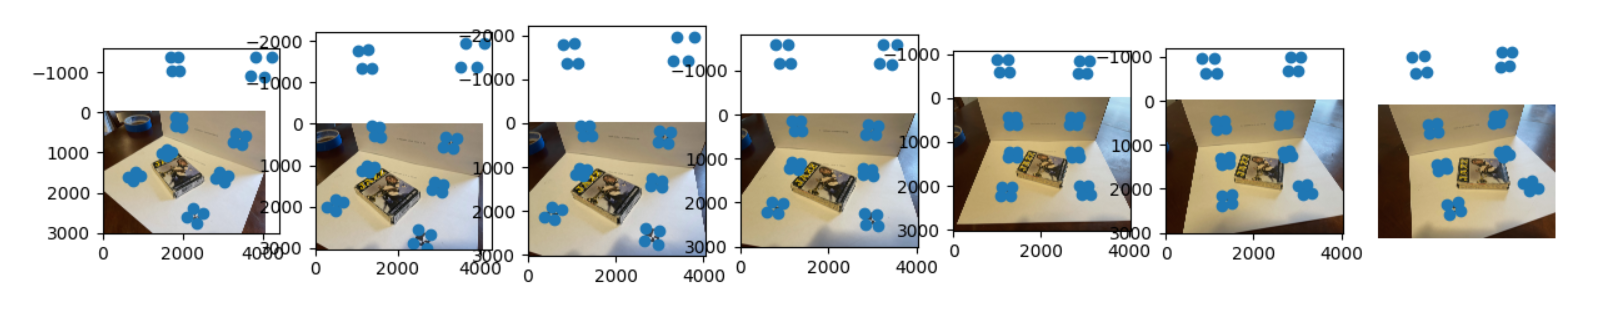
\includegraphics[width=\linewidth]{calculate_projection_matrix.png}
\end{figure*}

Result after implementing function \texttt{ransac\_fundamental\_matrix} for images 1 and 2 of sequences of cards.

\begin{figure*}[htbp]
    \centering
    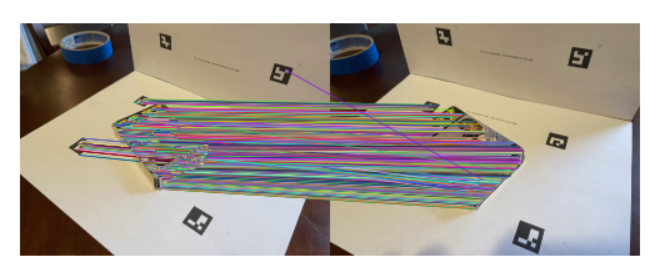
\includegraphics[width=0.8\linewidth]{ransac.png}
\end{figure*}

Show us an image of a 3D reconstruction of one of the sequences (mike and ikes, cards, or dollars). Discuss your observations of the effect of any remaining incorrect matches.

Below Left is the 3D reconstruction of cards. We could find that there are many mismatches in left side. By checking all the intermediate figures showing matches in 2D, we found that the markers can lead to many mismatches. As markers are rigidly placed across the images in certain direction, it might can partially explained why so many mismatch in one direction.
\begin{figure*}[htbp]
    \centering
    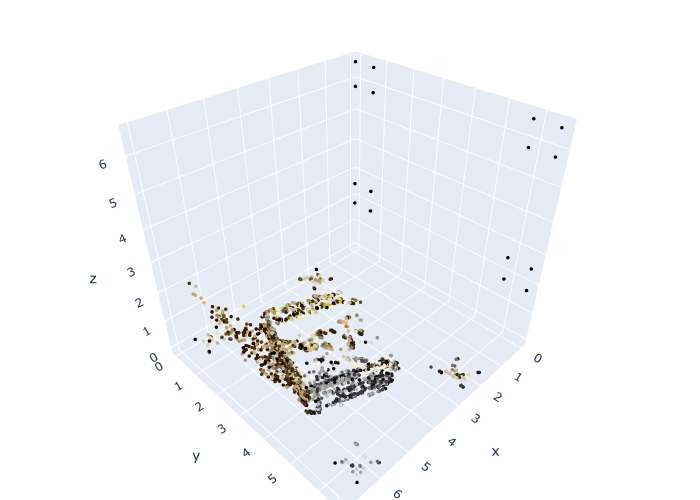
\includegraphics[width=0.49\linewidth]{cards.png}
    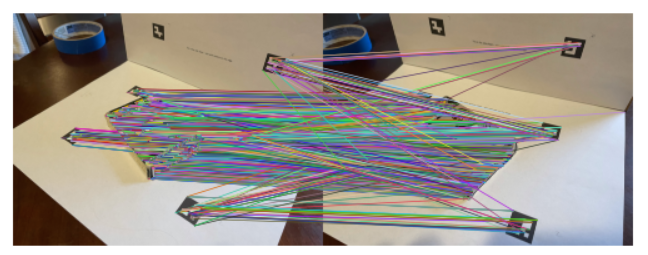
\includegraphics[width=0.49\linewidth]{mismatch.png}
\end{figure*}


\newpage
Write about your thoughts on how well RANSAC does. How does the number of iterations affect the output?

From the figure below, we could see that the number of iterations will affect the final number of matches in 3D spaces. Fewer number of iterations might not be able to find the best estimated fundamental matrix and thus, cannot find so many matches.
\begin{figure*}[htbp]
    \centering
    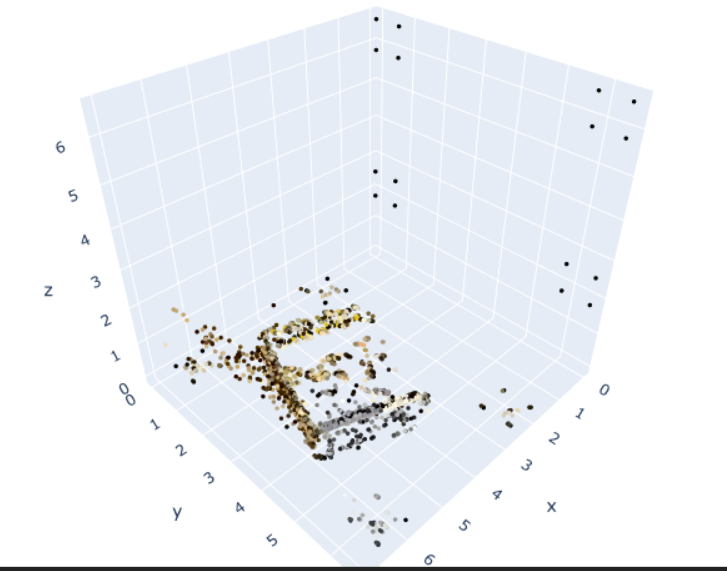
\includegraphics[width=0.49\linewidth]{iter1.png}
    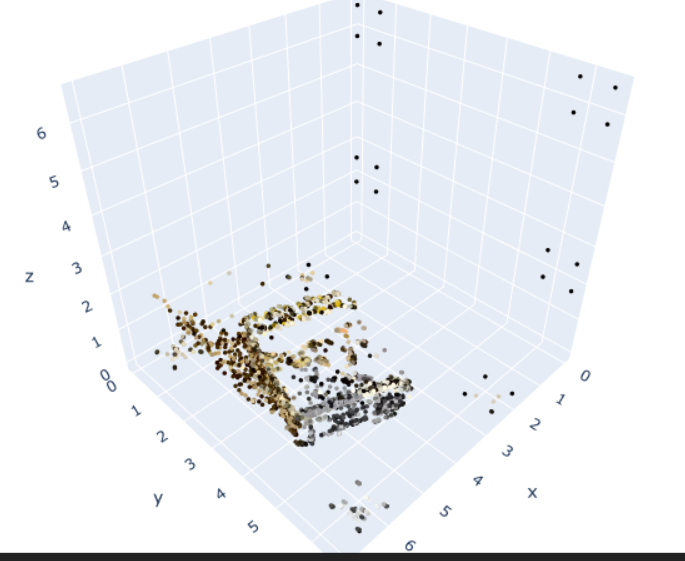
\includegraphics[width=0.49\linewidth]{iter100.png}
    \caption{\emph{Left}: the number of iteration in RANSAC is 1. \emph{Right}: the number of iteration in RANSAC is 100.}
\end{figure*}

\end{document}
